% CHAPTER 1
\chapter{WIND TURBINE MODELLING}
\label{chp:3}
Ancillary services are getting attention especially for renewable energy systems. Participation of renewable energy systems to frequency regulating mechanisms will be a necessity for the successful operation of the power system. Hence, the detailed modelling of renewable energy systems are essential for grid supporting implementations. In this chapter, detailed modelling for wind turbines is investigated. The wind turbine detailed modelling is presented for the wind turbines that are connected to grid with full-scale power electronics. 
\section{Wind Turbines with Full Scale Power Electronics}
The share of variable speed wind turbines with full scale power electronics is increasing worldwide due to the high efficiency. Full-scale power electronics enables the turbine to have wide speed range. The wind turbines in this type are able to adjust its speed according to the variation in the wind speed and torque \cite{Chen2009b}. PMSG wind turbines are one of the most common type of these turbines. Even though the price of the permanent magnet fluctuates with time, the reliability and high efficiency of this type of turbine increase its share in the market. The wind turbine modelling in this study is based on PMSG wind turbines. However, the ability to control the wind turbine output power is not just specific to PMSG wind turbines but the ones with full-scale power electronics. \par
Fig. \ref{varspeedpmsg_1}, \ref{varspeedpmsg_2} and \ref{varspeedpmsg_3} show the modelling of wind turbine topologies that are connected to grid full-scale back-to-back converter. In wind turbines with full-scale power electronics, stator of the wind turbine generator is not directly connected to grid. A back-to-back converter is used between generator and the electrical grid to ensure that the turbine speed is independent from the grid frequency. The back-to-back converter is composed of two converters to perform the AC/DC and DC/AC conversion. The converter which is connected to turbine generator is called Machine Side Converter (MSC) meanwhile the one connected to grid is called Grid Side Converter(GSC). Moreover, GSC is connected to grid with a filter in order to filter out high frequency currents due to switching action. Since GE2.75-103 model geared PMSG wind turbine model is used in this study, the turbine topology in Fig. \ref{varspeedpmsg_1} is emphasized. The turbine is composed of sub-models such as aerodynamic model, gearbox, PMSG, MSC and GSC. The details of the sub-models are given in the following sections.\par
\begin{figure}[h!]
	\centering
	\begin{subfigure}{0.9\textwidth} % width of right subfigure
		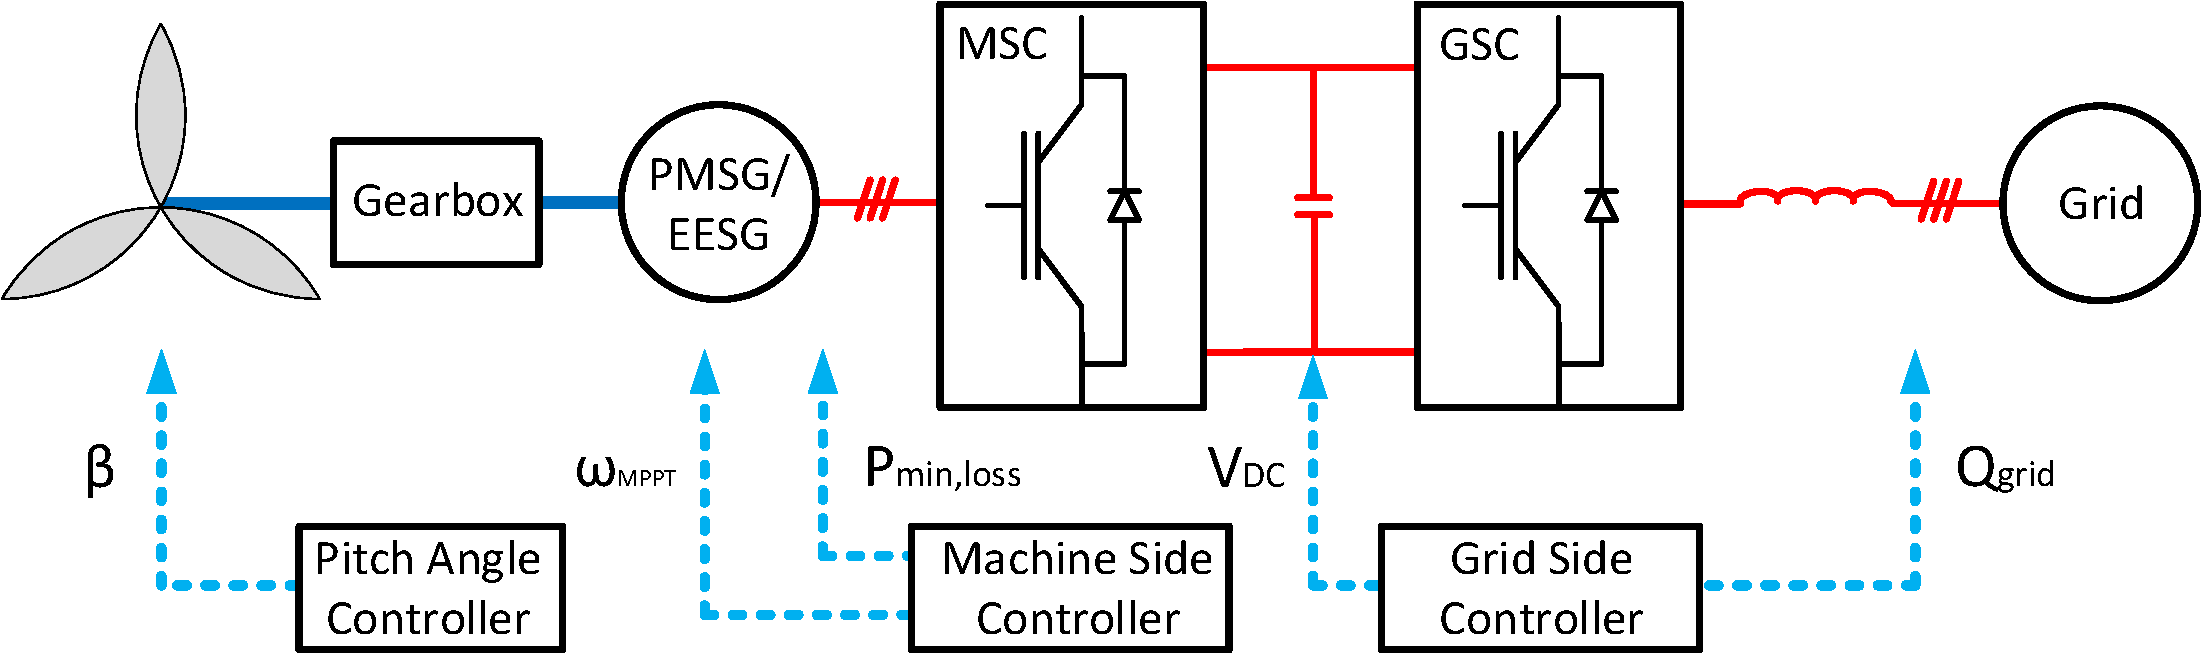
\includegraphics[width=0.9\linewidth]{windmodel2_1.pdf}
		\caption{Geared PMSG/EESG Wind Turbine}		
		\label{varspeedpmsg_1}
	\end{subfigure}
	\vspace{0.1em} % here you can insert horizontal or vertical space
	\begin{subfigure}{0.9\textwidth}
		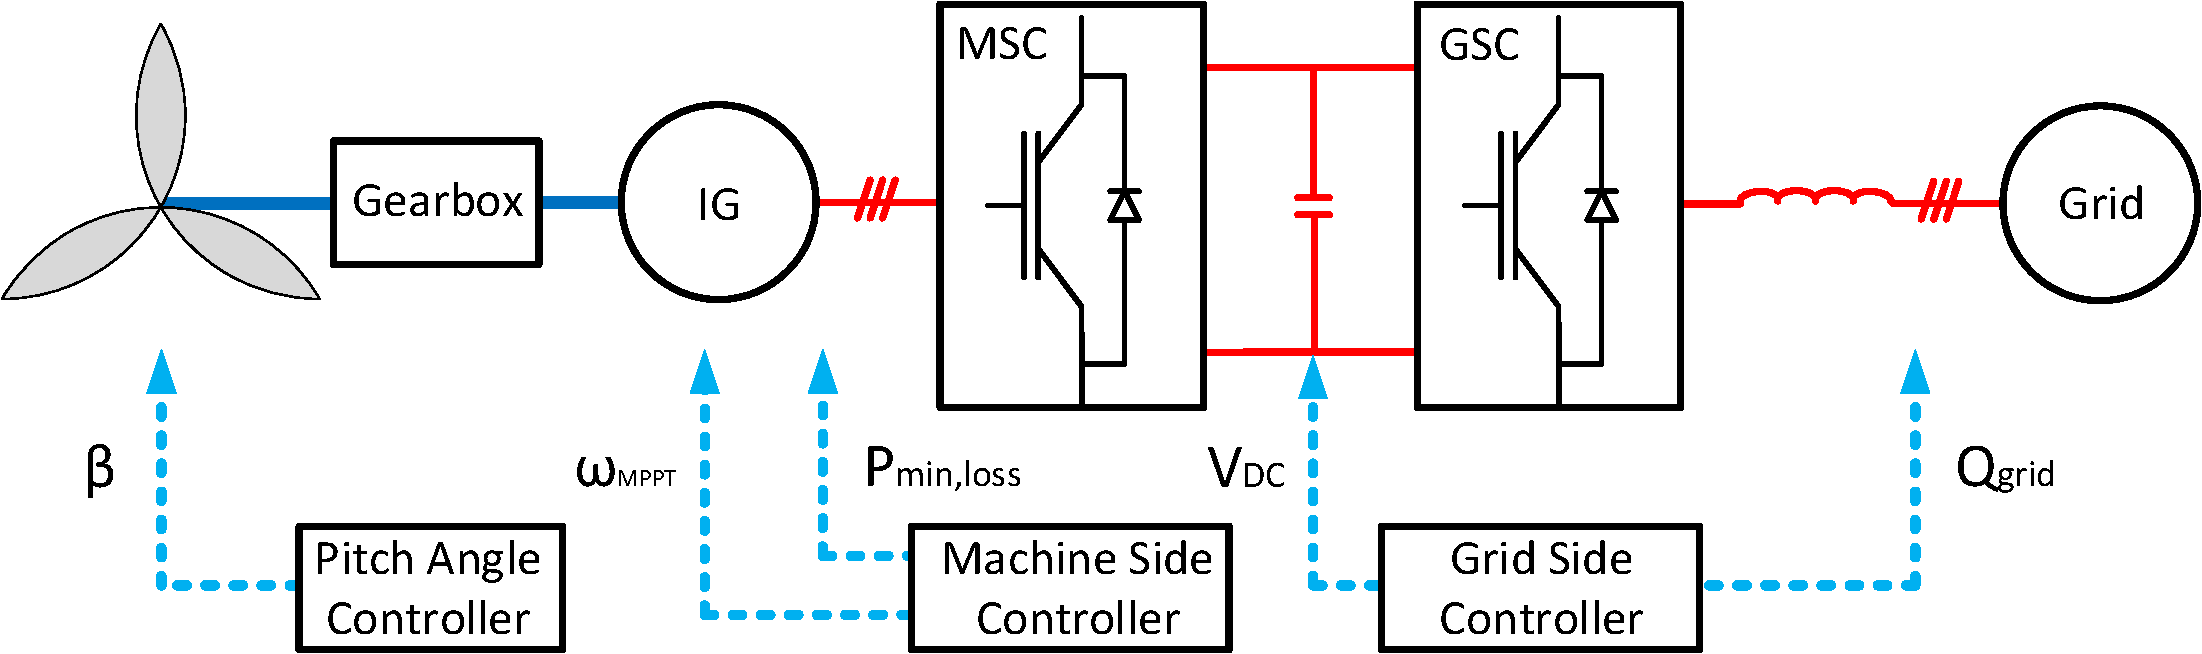
\includegraphics[width=0.9\linewidth]{windmodel2_2.pdf}
		\caption{Geared IG Wind Turbine}
		\label{varspeedpmsg_2}	
	\end{subfigure}
	\vspace{0.1em} % here you can insert horizontal or vertical space
	\begin{subfigure}{0.9\textwidth}
	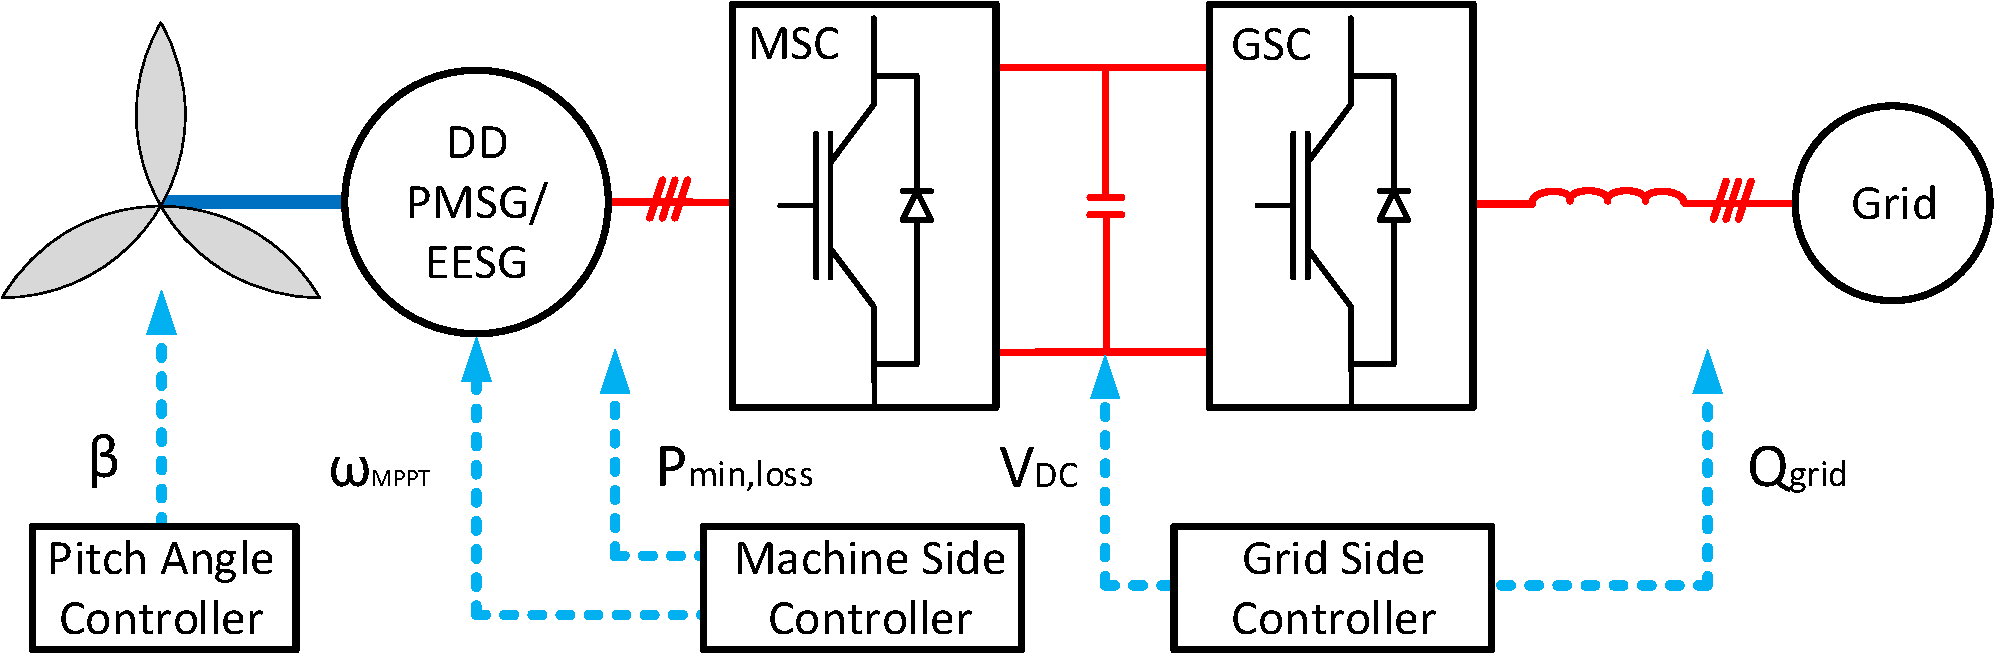
\includegraphics[width=0.9\linewidth]{windmodel2_3.pdf}
	\caption{Direct-Drive PMSG/EESG Wind Turbine}
	\label{varspeedpmsg_3}	
	\end{subfigure}
	\caption{Wind Turbine Topologies with Full-Scale Power Electronics}
\end{figure}
\subsection{Aerodynamic Model}
Aerodynamic model is the sub-model that captures power from the wind. The output of this block is the aerodynamic torque that rotates the turbine. However, the wind speed is not the only input. Turbine speed and pitch angle are also the inputs of the system since they affect the mechanical power that is captured from the wind.\par
The aerodynamic power of wind is given in Eq. (\ref{windpower}) where $\rho_{air}$ is air density in $kg/m^{3}$, $R$ is the blade radius in $m$ abd $v_{wind}$ is the wind speed in $m/s$. Note that this is the available power of the air that is striking the turbine swept area and it is not possible to extract that amount of energy. Otherwise, the air would be standstill behind the wind turbine \cite{Ackermann2005a}.
\begin{equation}
P_{wind}=0.5\rho_{air}\pi R^{2} v_{wind}^{3}
\label{windpower}
\end{equation}
The wind turbine captures a fraction of the available wind power that is denominated as power coefficient $C_{p}$. Therefore, turbine power captured from wind can be found with the Eq. (\ref{turbinepower}).
\begin{equation}
P_{tur}=C_{p}P_{wind}
\label{turbinepower}
\end{equation}
Power coefficient determines the amount of power to be captured from wind and it is a non-linear function of the tip speed ratio, $\lambda$ and pitch angle, $\beta$. Tip speed ratio is a parameter proportional with turbine speed. It can be defined as the ratio of the speed in the turbine tip to the wind speed as in the Eq. (\ref{tipspeed}). Power coefficient for a specific tip speed ratio and pitch angle can be found with the Eq. (\ref{cp}) and (\ref{lambdai}) where $c_{1}$ is 0.5176, $c_{2}$ is 116, $c_{3}$ is 0.4, $c_{4}$ is 5, $c_{5}$ is 21 and $c_{6}$ is 0.0068 \cite{Heier}.\par
\begin{equation}
\lambda=\frac{\omega_{tur}R}{v_{wind}}
\label{tipspeed}
\end{equation}
\begin{equation}
C_{p}(\lambda,\beta)=c_{1}(c_{2}/\lambda_{i}-c_{3}\beta-c_{4})e^{-c_{5}/\lambda{i}}+c_{6}\lambda
\label{cp}
\end{equation}
\begin{equation}
\frac{1}{\lambda_{i}}=\frac{1}{\lambda+0.08\beta}-\frac{0.035}{\beta^{3}+1} 
\label{lambdai}
\end{equation}
\begin{figure}[h!]
	\centering
	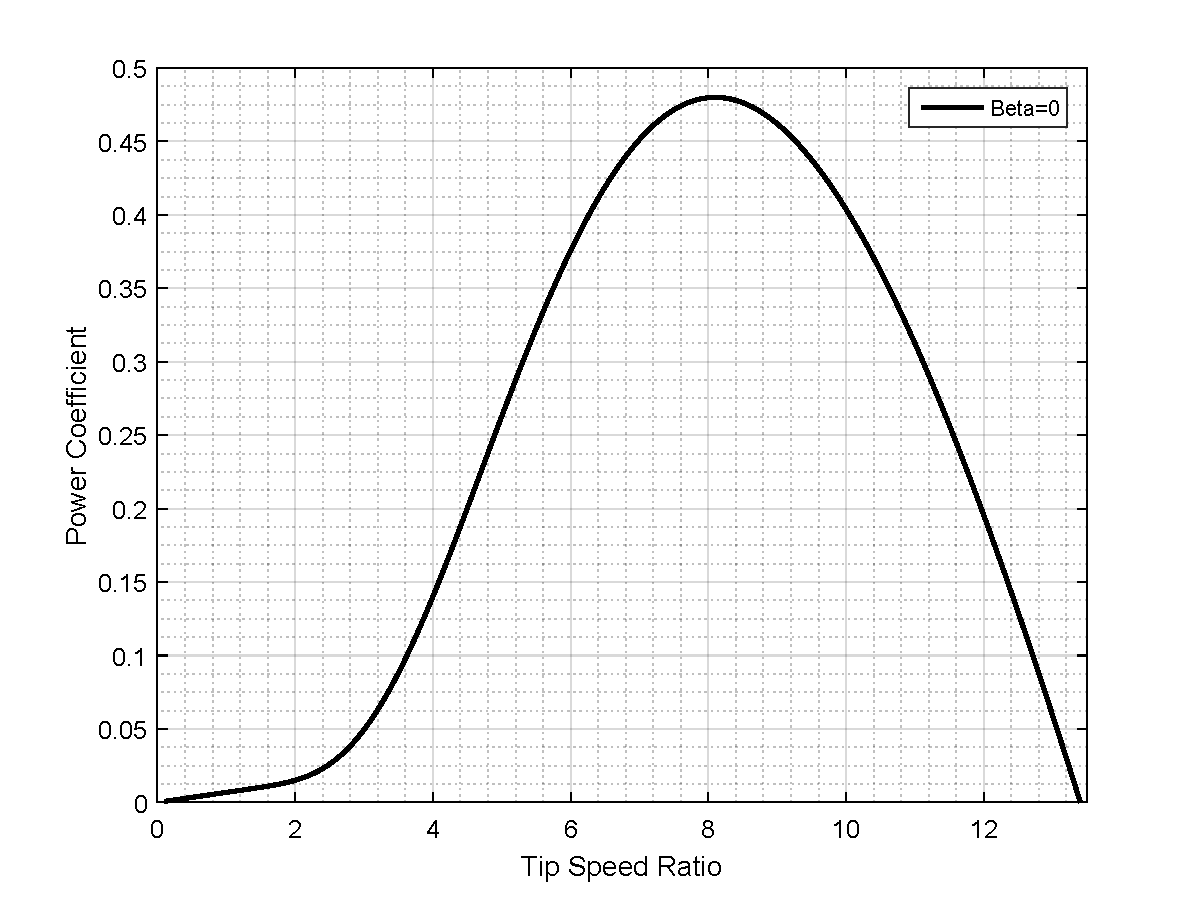
\includegraphics[width=.95\linewidth]{PowerCoefficient.pdf}
	\caption{Power Coefficient Variation with Tip Speed Ratio under Zero Pitch Angle}
	\label{variationofcp}
\end{figure} 
\par
Variation of power coefficient $C_{p}$ is given in Fig. \ref{variationofcp} for varying tip speed ratio. For the zero pitch angle, power coefficient has the maximum value of 0.48 for the tip speed ratio of 8.1. In order to ensure that the maximum of wind power is extracted, wind turbine should rotate a speed that gives the optimum tip speed ratio. This is ensured by the Maximum Power Point Tracking (MPPT) algorithms. 
\subsubsection{Maximum Power Point Tracking Algorithms}
In the literature, different methods are presented in order to operate in the Maximum Power Point. Perturb\&Obserb (P\&O) is the most common MPPT method in the literature \cite{Wang2004}, \cite{Barakati2009}. The methods simply creates a perturbation in the generator speed. The change in the generator speed creates also change in the active power output. If the power is increased with this perturbation, the generator speed is again perturbed in the same direction until a decrease in the active power is observed. This methods is the simplest method and does not require any calculation or wind speed measurement. However, the algorithm creates oscillations in the generator speed and active power. This method is also called as Hill-Climb Search (HCS) method in the literature.\par
Another MPPT algorithm is the wind speed measurement method \cite{Thriringer1993}, \cite{C.A.2013}. If the wind speed is estimated accurately, the optimal generator speed can be calculated. However, wind speed estimation is complicated and increases the cost. Another commonly used MPPT algorithm is the power-signal feedback (PSF) control \cite{C.A.2013},\cite{Wang2004}, \cite{Lu2002}. This method requires maximum power curve of the wind turbine based on the experimental results. A look-up table is constructed with obtained wind turbine speed and active output power values. However, using generator speed and active power measurements is the main drawback of this algorithm. Finally, there are numerous number of much complex MPPT algorithms based on fuzzy-logic \cite{Zeng2008} or neural-network \cite{Lin2011}. However, these MPPT algorithms are out of scope of this thesis. Therefore, optimal generator speed is provided in this study according to the wind speed. 
\subsubsection{Pitch Angle Control}
According to Eq. (\ref{windpower}), wind power increases with the cube of the wind speed. Hence, wind power increases dramatically for the high wind speeds. In order to decrease power, pitch angle i.e. blade angle is increased. Since the power coefficient, $C_{p}$ is a function of the pitch angle, $\beta$, wind power can be curtailed with increased blade angle. Variation of power coefficient for two different pitch angle is shown in Fig. \ref{cpwithtwopitchangle}. Increasing pitch angle by $1.176^{\circ}$ decreases power coefficient by 10\%.\par
\begin{figure}[h!]
	\centering
	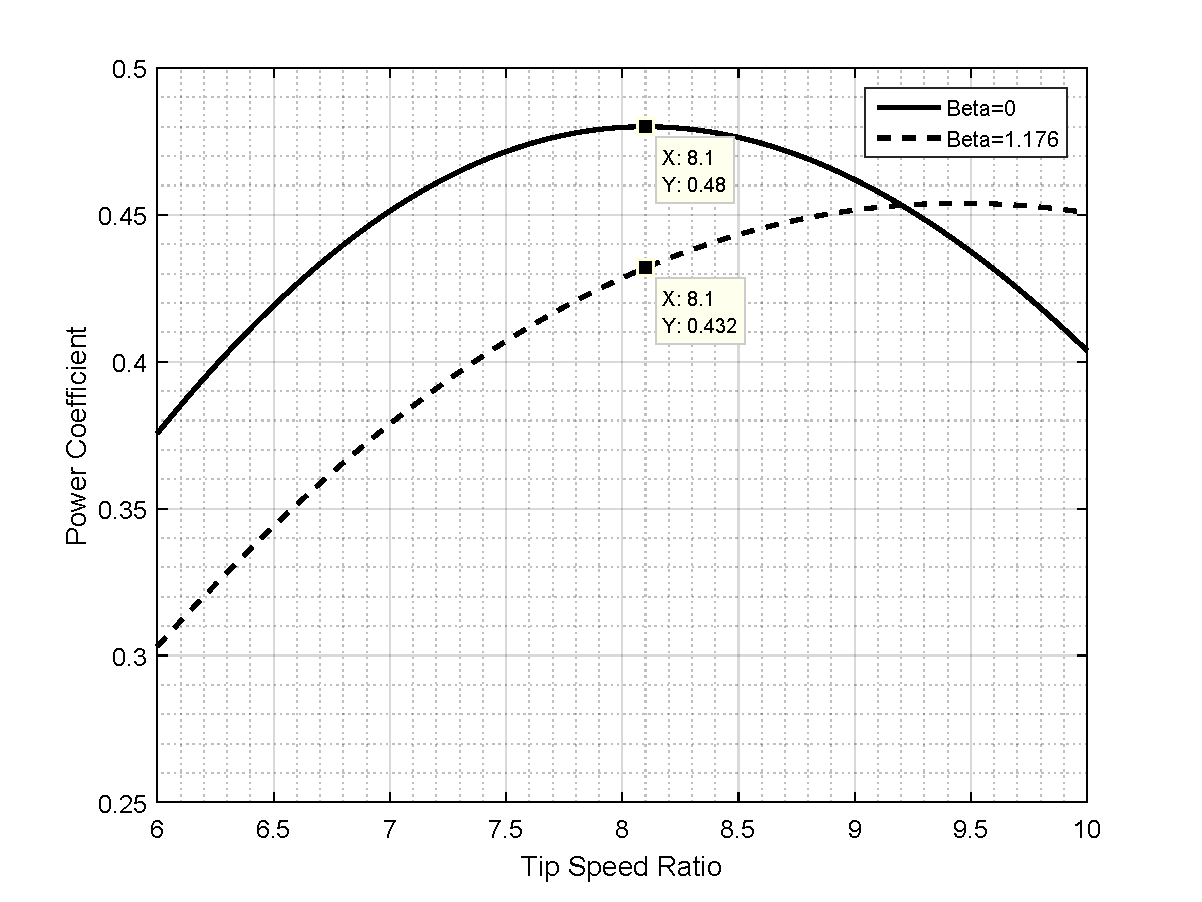
\includegraphics[width=.95\linewidth]{powercoefficient_with_varying_pitch.pdf}
	\caption{Power Coefficient Variation for Two Different Pitch Angle}
	\label{cpwithtwopitchangle}
\end{figure} 
As long as wind power is below the rated power, the wind turbine is operated in MPPT speed. This is ensured by obtaining optimal tip speed ratio. This means that for zero pitch angle, MPPT speed is increased linearly with wind speed. Before reaching rated power, MPPT speed might reach maximum generator speed. In this case, wind turbine reference speed will be the maximum generator speed. However, turbine speed cannot be decreased down to reference speed when the torque limit is reached. Hence, the pitch angle should be increased to regulate the turbine speed. Pitch angle controller is depicted in Fig. \ref{pitchcontroller}. Notice that the pitch angle is increased when the speed exceeds maximum generator speed. Otherwise, the pitch angle kept as zero.\par
\begin{figure}[h]
	\centering
	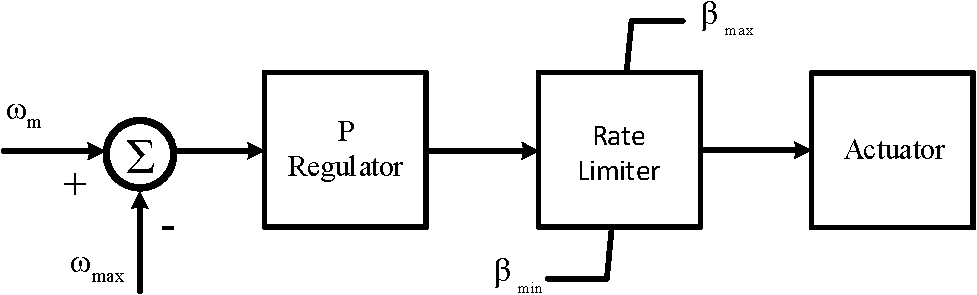
\includegraphics[width=.8\linewidth]{pitchcontroller2.pdf}
	\caption{Pitch Angle Control Diagram}
	\label{pitchcontroller}
\end{figure}
The responsibility of the pitch angle controller is the regulation of the blade angle but each blade in the wind turbine is a few tonnes. Therefore, the blade angle cannot be changed instantaneously and limited with rate limiter. The rate of change of pitch angle in this study is limited with $10^{\circ}/s$ \cite{Ackermann2005a}. Besides, the pitch angle controller takes action as soon as the maximum generator speed is exceeded. Therefore, wind turbine operation deviates from optimal tip speed ratio. This can also be observed from the variation of power coefficient, $C_{p}$ with the wind speed for the wind turbine GE 2.75-103 used in this study. Variation of the $C_{p}$ is shown in Fig. \ref{powercoefficientge}.
\begin{figure}[h!]
	\centering
	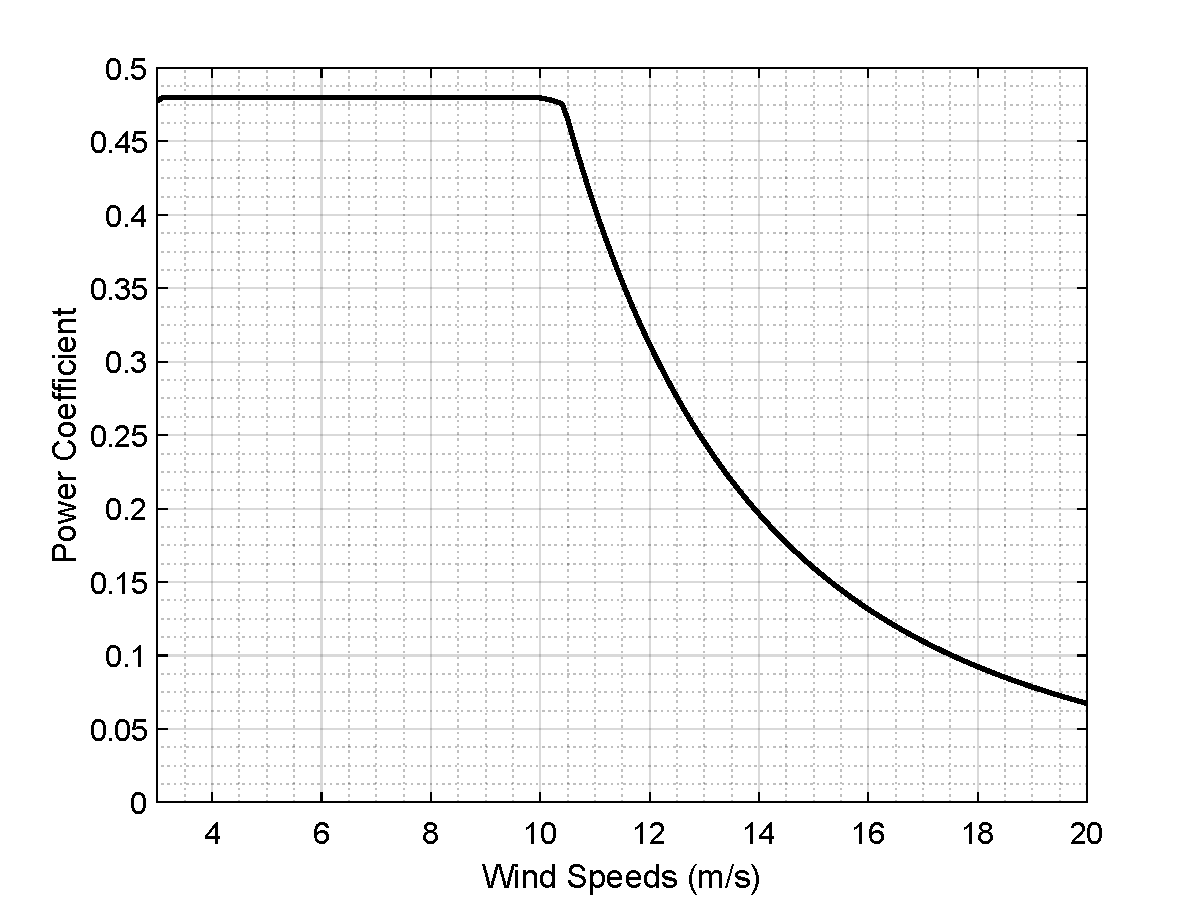
\includegraphics[width=.9\linewidth]{cp_wind.pdf}
	\caption{Power Coefficient Variation for GE 2.75-103}
	\label{powercoefficientge}
\end{figure}
\subsection{Gearbox}  
Variable speed PMSG wind turbines have a gearbox between turbine and generator except for direct-drive wind turbines. The gearbox increases angular speed and decreases the torque in the generator side. By decreasing the rated torque, generator size and cost can be reduced since the generator size is almost proportional to rated torque due to constant shear stress \cite{Polinder2013aa}. Moreover, turbine speed is increased to the allowable speed range of the generator which is generally much higher than that of wind turbines. Otherwise, generator should have high pole numbers. \par
A gearbox model is depicted in Fig. \ref{gearboxmodel}. They are mainly used for speed and torque conversion. It should be noted that the gearboxes are lossy systems. Therefore, the output torque of the gearbox would be lower than the ratio of input torque to gearbox conversion ratio. Direct-drive systems are based on the elimination of the gearbox systems by direct connection between turbine and generator in order to increase efficiency and reliability \cite{Chen2009b}. In this study, 3 stage (1 planetary / 1 helical) gearbox is modelled with \%97 efficiency \cite{UKONSAARI2016}. 
\begin{figure}[h!]
	\centering
	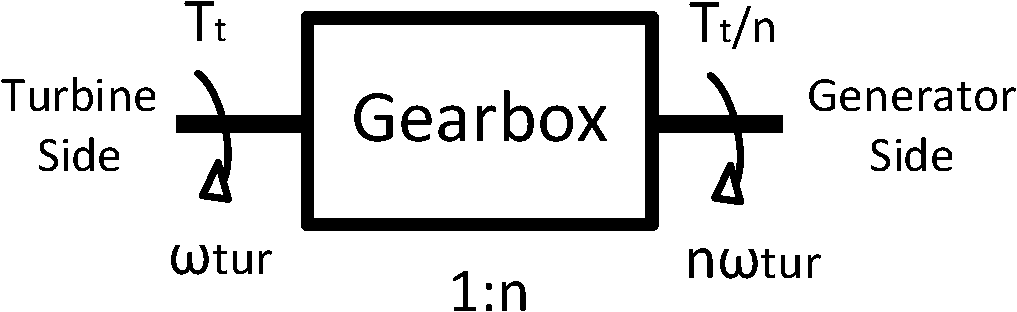
\includegraphics[width=.5\linewidth]{gearbox.pdf}
	\caption{Gearbox Modelling}
	\label{gearboxmodel}
\end{figure}
\subsection{Permanent Magnet Synchronous Generator}
\label{pmsgsection}
PMSGs and electrically excited generators can be employed with full-scale power electronics. However, PMSGs are generally preferred over electrically excited synchronous generators due to their high efficiency. The absence of electrical excitation on the rotor decreases losses. Besides, slip ring is not needed in the generator which also increases the reliability of the PMSG wind turbines. Dynamical equations of the salient pole PMSG are projected on a reference frame which rotates synchronously with magnet flux and given in Eq. (\ref{v1d}) and (\ref{v1q}) where $R_{1}$ is stator resistance in $\Omega$, $L_{sd}$ and $L_{sq}$ are d and q axis inductances in $H$, $i_{ad}$ and $i_{aq}$ are d and q axis currents in $A$, $\omega$ is the electrical angular frequency in $rad/s$, $\psi_{f}$ is magnet flux linkage in $Vs$ \cite{Ackermann2005a}. 
\begin{equation}
v_{1d}=R_{1} i_{ad}+L_{sd}\frac{di_{ad}}{dt}-L_{sq}\omega i_{sq}
\label{v1d}
\end{equation}
\begin{equation}
v_{1q}=R_{1} i_{aq}+L_{sq}\frac{di_{aq}}{dt}+L_{sd}\omega i_{sd}+\omega \psi_{f}
\label{v1q}
\end{equation}
Another important PMSG parameter is the power in dq frame. The power expression is given in Eq. (\ref{pmsgpower}). The electromechanical torque can be found by the relation between power and angular speed. The torque expression is also given in Eq. (\ref{pmsgtorque}) where p is the number of pole pair.
\begin{equation}
P_{elm}=\frac{3}{2}\omega i_{aq} (\psi_{f}+i_{ad}(L_{sq}-L_{sd}))
\label{pmsgpower}
\end{equation}
\begin{equation}
T_{e}=\frac{P_{elm}}{w_{m}}=\frac{P_{elm}}{w/p_{p}}=\frac{3}{2}p_{p} i_{aq} (\psi_{f}+i_{ad}(L_{sq}-L_{sd}))
\label{pmsgtorque}
\end{equation}

Given equations are defined for salient pole machines. If the clyndrical rotor machine is used, the torque equation reduces to the Equation \ref{pmsgtorque2}.
\begin{equation}
T_{e}=\frac{3}{2}p_{p} i_{aq} \psi_{f}
\label{pmsgtorque2}
\end{equation}
\subsection{Machine Side Converter}
Variable speed wind turbines that are equipped with the back-to-back converters are able to decouple grid frequency and the turbine speed. This gives wind turbine degree of freedom for the rotational speed. In this way, turbine is able to capture the maximum available power from wind. Machine Side Converter (MSC) i.e. Generator Side Converter is the converter that is connected between generator and DC-bus. The three phase generator output AC voltage is converted to DC voltage. Conversion from AC to DC can be achieved by three-leg full bridge converters. This converter can be equipped with uncontrolled, semi-controlled and fully-controlled switches. Fully-controlled switches such as MOSFET,IGBT are commonly used in the industry and gives two control parameters to the user. \par
Voltages and currents are generally transformed into synchronously rotating reference frame or also called dq frame. Since the frame is rotating in synchronous speed, three-phase phasors are transformed to DC quantities. Therefore, its control becomes easier \cite{Kazmierkowski2002}. Proportional-integral (PI) controllers are associated with the dq control structure due to their satisfactory behaviour interaction to DC variables \cite{Blaabjerg2006a}. Hence, the control in the back-to-back converter is achieved with PI controllers in the dq frame. \par
\begin{figure}[h!]
	\centering
	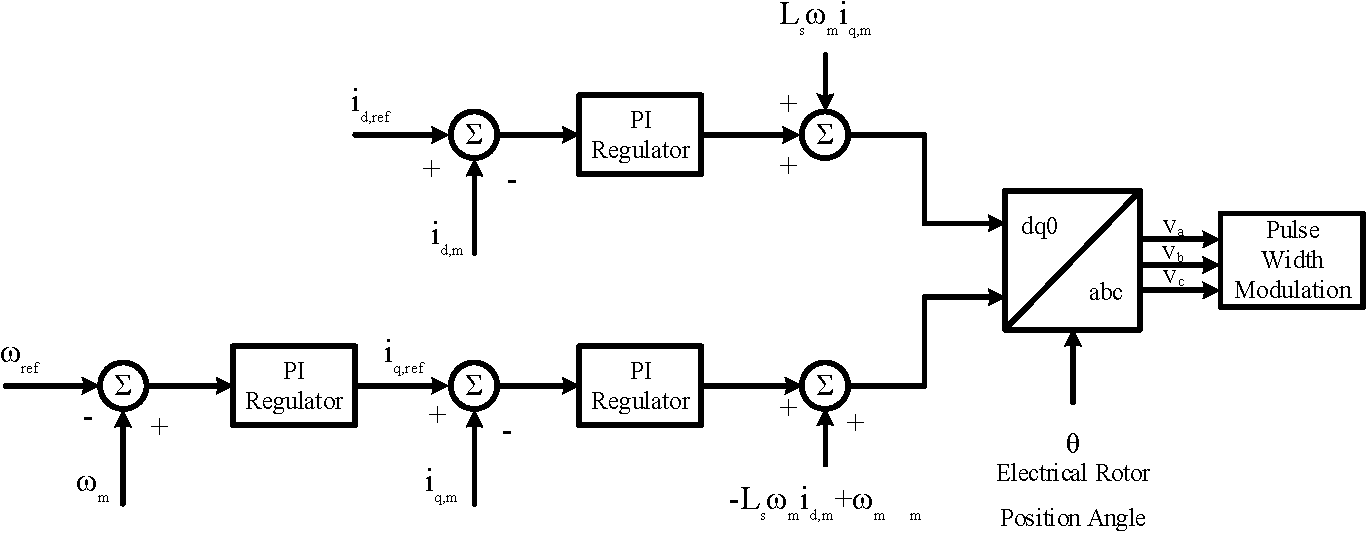
\includegraphics[width=.95\linewidth]{msc.pdf}
	\caption{Machine Side Controller Diagram}
	\label{msc}
\end{figure}
The control diagram of the MSC is depicted in Fig. \ref{msc} according to the study in \cite{Chinchilla2006}. In dq frame, it is possible to control two parameters. One of these parameters is the d-axis current that is set zero in order to decrease the stator copper losses. The other parameter is the q-axis current that is proportional to the electromagnetic torque as it can be observed in the Eq. (\ref{pmsgtorque2}). However, q-axis current or torque is controlled in order to regulate the turbine speed. Therefore, turbine speed is adjusted such that the turbine will capture maximum available power in the wind. 
\subsection{Grid Side Converter}
Grid Side Converter (GSC) or Line Side Converter (LSC) is the converter that is connected between DC-link capacitor and grid. GSC works as an inverter that injects current synchronous to grid. Currents and voltages are transformed into synchronously rotating frame that is aligned with the grid voltage. Therefore, d-axis current determines the amount of current which is in phase with the grid voltage meanwhile q-axis current determines amount of current that is out of phase with the grid voltage. In other words, injecting d-axis current injects active power to grid meantime q-axis current injects reactive power to grid.\par
The responsibility of the GSC is regulating DC voltage and the reactive power injected to the grid. The control diagram of the GSC is given in Fig. \ref{gsc}. As seen from the figure, DC-bus voltage is regulated by controlling the d axis current. If the DC-bus voltage increases above the reference value, d-axis current reference is increased. As a result, active power increases. Increased active power also decreases the DC-bus voltage level. Reference value of the q-axis current is set to zero in normal operation, consequently unity power factor. For Low Voltage Ride-Through studies, q-axis current is determined according to the reactive power value requirement. \cite{Orowska-Kowalska2014} \par
\begin{figure}[h!]
	\centering
	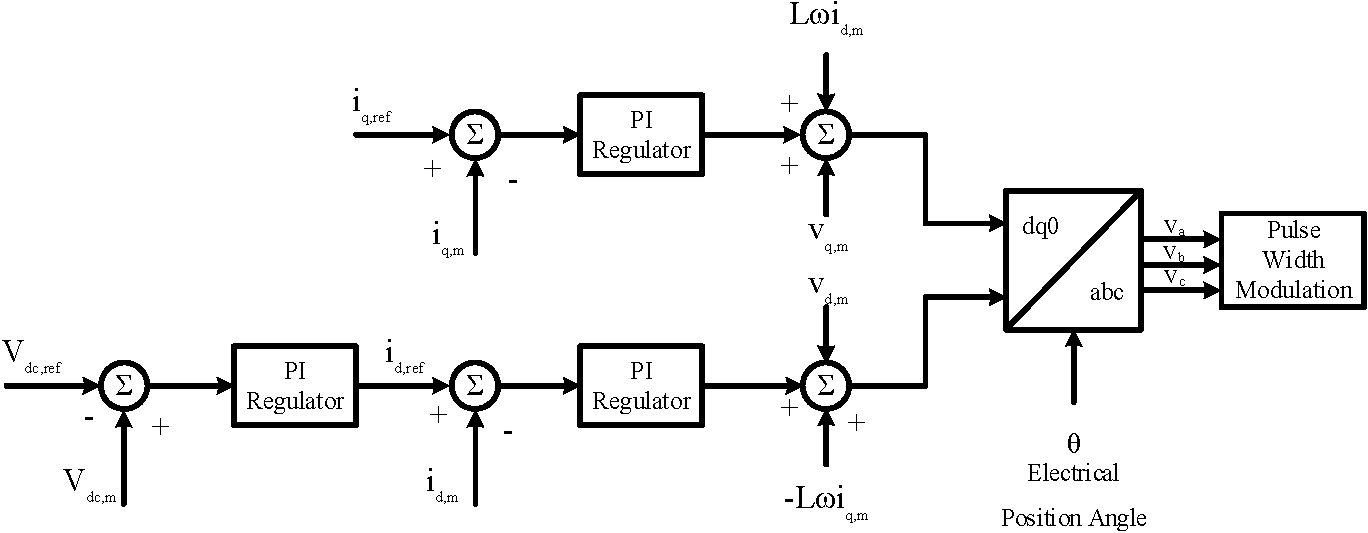
\includegraphics[width=.98\linewidth]{gsc.pdf}
	\caption{Grid Side Controller Diagram}
	\label{gsc}
\end{figure}
GSC is connected to grid through a filter. Therefore, the output voltage of the converter is not equal to the that of grid. The relation between converter voltage, grid voltage and current is derived through Eq. (\ref{crossilk}) to (\ref{crosscomp2}) where $v_{c}$ is the converter voltage, $v_{g}$ is the grid voltage and  $i_{g}$ is the grid current measured in the grid side. As it is observed in Eq (\ref{crosscomp1}) and (\ref{crosscomp2}), converter side voltage includes same axis grid voltage and a term proportional to cross axis current which is called cross-coupled term. Therefore, the outputs of the inner PI regulators are compensated and forwarded to Pulse Width Modulation after transformation to three-phase voltages.
\begin{equation}
\overline{v_{c}}=v_{dc}+jv_{qc}
\label{crossilk}
\end{equation}
\begin{equation}
\overline{v_{g}}=v_{dg}+jv_{qg}
\end{equation}
\begin{equation}
\overline{i_{g}}=i_{dg}+ji_{qg}
\end{equation}
\begin{equation}
\overline{v_{c}}=\overline{v_{g}}+\overline{i_{g}}j\omega L
\end{equation}
\begin{equation}
v_{dc}+jv_{qc}=v_{dg}+jv_{qg}+j\omega L (i_{dg}+ji_{qg})
\end{equation}
\begin{equation}
v_{dc}=v_{dg}-\omega L i_{qg}
\label{crosscomp1}
\end{equation}
\begin{equation}
v_{qc}=v_{qg}+\omega L i_{dg}
\label{crosscomp2}
\end{equation}
The PI regulators of the wind turbine model is tuned with trial error method. In this study, the modelled wind turbine is connected to grid with an L filter even though the actual turbine is connected to grid with an LCL filter. However, the actual system would operate better than the modelled case since the the LCL filter has superior performance than L filters \cite{Brantsater2015}. Nonetheless, L filter has provided sufficient performance for the successful operation of the wind turbine in this study regardless from the power quality standards in the output current. The active power of the wind turbine under varying wind speed is given in the Fig. \ref{powerdata}. \par
\begin{figure}[h!]
	\centering
	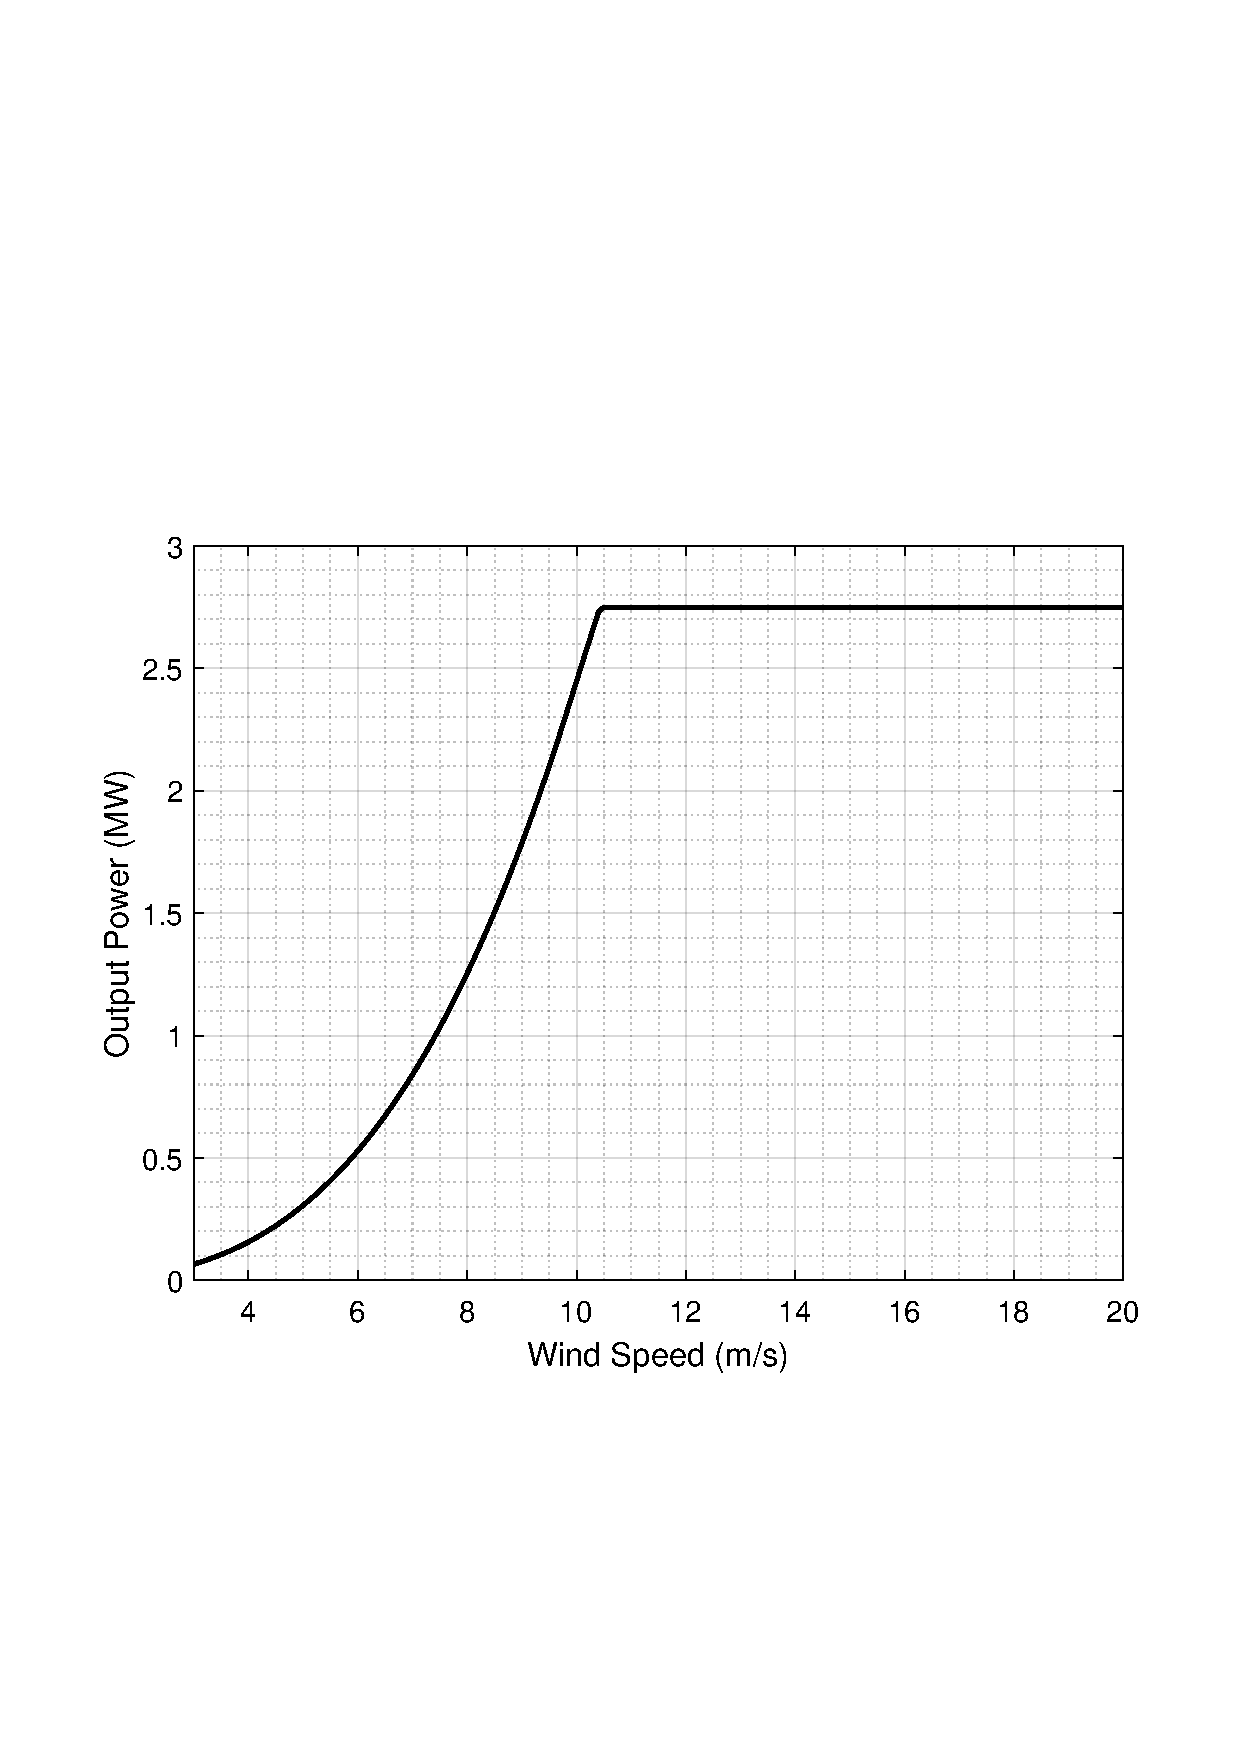
\includegraphics[width=.9\linewidth]{powerdata.pdf}
	\caption{Variation of the Active Power of the Wind Turbine}
	\label{powerdata}
\end{figure}
\section{Synthetic Inertia Implementation}
As explained Section \ref{swing}, synchronous generators change their speed according to the balance between input mechanical and electromechanical powers. Furthermore, if the frequency changes, the electromechanical power of the generators also change. Nonetheless, the renewable energy systems which are connected to grid with a power electronics interface are unresponsive to the deviations in the grid frequency.\par
The definition of the synthetic inertia is the controlled contribution of electrical torque that is proportional to RoCoF in the unit connection terminal \cite{Eriksson2017}. Synthetic inertia (also called as 'virtual inertia') is the method that emulates the synchronous generator in the renewable energy systems. In this method, the active power output of the wind turbines are adjusted according to the Eq. (\ref{synthetic}) where $H_{syn}$ is the synthetic inertia constant in seconds and $\omega_{t}$ is the terminal angular frequency in pu. The increase in the active power is proportional to RoCoF as well as the emulated inertia constant. The emulated inertia constant can be different from the inertia constant of the renewable energy system. For instance, the solar PV systems does not have inertia. Even in these systems, an inertia constant can be emulated as long as the system includes stored energy. In the wind turbines, the additional energy can be yielded from the kinetic energy in the turbine inertia. For solar PV systems, energy storage systems or the store energy in the DC-link capacitor can be utilized.\par
\begin{equation}
\Delta P_{e}=-2H_{syn}\frac{d\omega_{t}}{dt}\omega_{t}
\label{synthetic}
\end{equation}
In order to implement synthetic inertia in the system, a relation between frequency and active power of the wind turbine should be constructed. Wind turbine in this study is variable speed wind turbine with full scale power electronics. The speed of the turbine is controlled by MSC such that active power is adjusted. Inertial support modification is depicted in Fig. \ref{modifiedmsc}. The new value of the active power is determined according to the swing equation. However, the wind turbine in this study is operated with a reference speed rather than a reference power. Therefore, the assigned power value should be used in order to yield the q-axis current reference value. Reference q-axis current is derived between the Eq. (\ref{inertialsupport1}) to Eq. (\ref{inertialsupport4}).\par
\begin{figure}[h!]
	\centering
	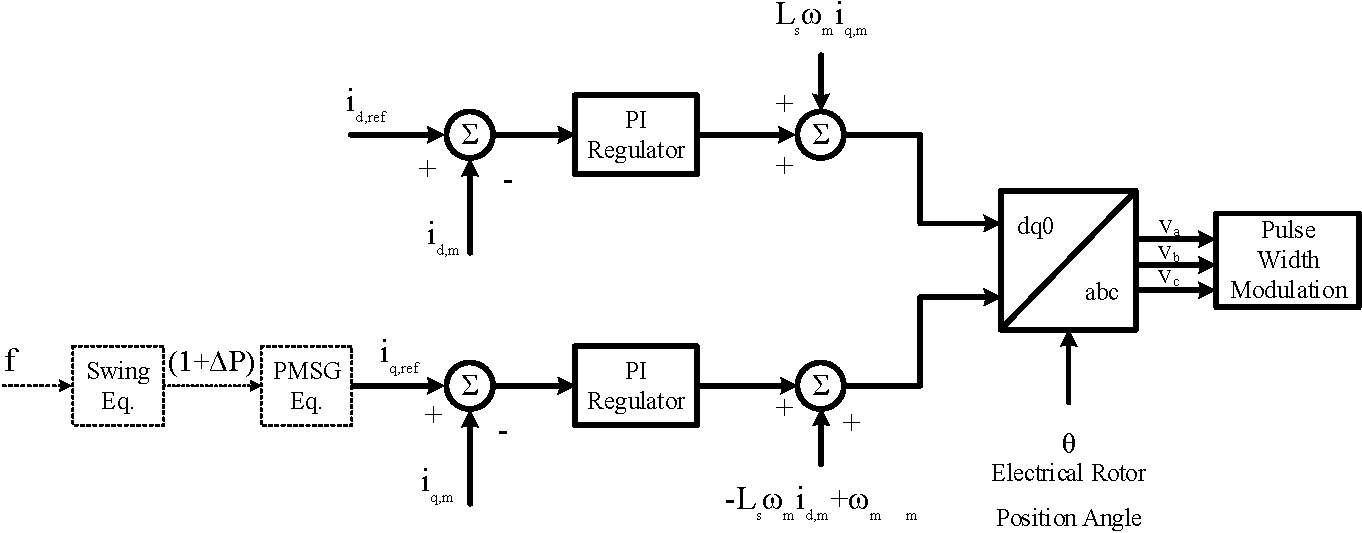
\includegraphics[width=.98\linewidth]{msc_modified.pdf}
	\caption{Modified MSC for Inertial Support}
	\label{modifiedmsc}
\end{figure}
\begin{equation}
P_{new}=(1+\Delta P) P_{pre}
\label{inertialsupport1}
\end{equation}
\begin{equation}
T_{new} \omega_{m}=(1+\Delta P) T_{pre} \omega_{pre}
\label{inertialsupport2}
\end{equation}
\begin{equation}
\frac{3}{2} p_{p} \psi_{f} i_{q,new} \omega_{m}=(1+\Delta P) \frac{3}{2} p_{p} \psi_{f} i_{q,pre} \omega_{pre}
\label{inertialsupport3}
\end{equation}
\begin{equation}
 i_{q,ref}=i_{q,new}=(1+\Delta P) \frac{i_{q,pre} \omega_{pre}}{ \omega_{m}} 
\label{inertialsupport4}
\end{equation}
\subsection{Synthetic Inertia Activation Schemes}
Another issue about inertial support is the time instant to trigger synthetic inertia. In the literature, continuous operation, under-frequency trigger and maximum-frequency gradient are discussed \cite{Gonzalez-longatt2015}. It is obvious that continuous operation would create oscillations in active power output due to the continuous deviations in grid frequency. This is an unrealistic operation and is used for comparison purposes.\par
Second activation method is the under-frequency trigger which is the activation when the frequency decreases below a threshold value. It can be used for capturing the time instant for the inertial support. However, power grid might be in a stable point even if the frequency is 49.8Hz. Therefore, this method would be unsuccessful depending on the disturbance event. \par 
Third activation scheme is the maximum-frequency gradient trigger. It uses a controller that is very similar to RoCoF relays and tracks the frequency gradient. Once the frequency gradient is below a threshold value, the synthetic inertia is activated. Since the severity of frequency disturbance event is related to the RoCoF, this activation scheme is the most remarkable scheme \cite{Gonzalez-longatt2015}. \par The activation of the inertial support by only frequency-gradient (RoCoF) might be misleading. For instance, a negative RoCoF value when the frequency is above the nominal value is not a frequency disturbance. Therefore, the inertial support should not be activated unless the frequency is below a threshold. Thus, in this study, maximum-frequency gradient is used in coordination with the under-frequency trigger. \par 
Grid RoCoF changes in the grid according to the disturbance level as well as the grid inertia. According to the disturbances in the Continental Europe System within the last 15 years, RoCoFs in the range between 0.1Hz/s and 1Hz/s are observed \cite{ENTSO-E2016}.Therefore in this study, 0.1Hz/s of RoCoF threshold with a frequency dead-band of 10mHz is selected. In this way, a negative RoCoF above 49.99Hz is not captured as events as long as it does not decrease below the under frequency threshold.
\subsection{Source of the Inertial Support}
The renewable energy systems cannot determine the amount of power in contrast the conventional systems. A thermal power plant, for instance, adjusts its power output as desired. However, the source of power in renewable energy is intermittent due to nature of the power source. This is why a spare energy is required in order to change the power output.\par
The stored energy in a wind turbine exists in the generator and turbine inertia. Therefore, the drive train of the wind turbine is important for the stored energy in the turbine. Different drive train concepts are compared in Table \ref{gencompare} according to the typical generator data presented in \cite{Seman2011}. According to the typical generator data and typical gearbox ratios, the stored energy with the High Speed Full Converter (HSFC) is calculated as 16.2MJ meanwhile DFIG concept stored 15.7MJ. However, the Direct-Drive concept stores 13.6MJ energy. Even though the stored energies close to each other, it is observed that the higher speed generator concepts store more than that of lower speed concepts. Notice that the wind turbine studied in thesis is a 3 stage HSFC wind turbine which store the highest energy compared to the other drive trains in the same power class.
% Please add the following required packages to your document preamble:
% \usepackage{graphicx}
\begin{table}[h!]
	\centering
	\resizebox{\textwidth}{!}{%
		\begin{tabular}{|c|c|c|c|c|}
			\hline
			\textbf{\begin{tabular}[c]{@{}c@{}}Drive\\   Train Concept\end{tabular}}       & \begin{tabular}[c]{@{}c@{}}Doubly-Fed \\ 3 Stage Gear\end{tabular} & \begin{tabular}[c]{@{}c@{}}Low Speed\\ Full Converter \\ (LSFC)\\   Direct Drive\end{tabular} & \begin{tabular}[c]{@{}c@{}}Medium Speed\\ Full Converter\\   (MSFC) \\ 2 Stage Gear\end{tabular} & \begin{tabular}[c]{@{}c@{}}High Speed\\ Full Converter\\  (HSFC)\\ 3 Stage Gear\end{tabular} \\ \hline
			\textbf{Generator Type}                                                        & DFIG                                                               & PMSG                                                                                          & PMSG                                                                                             & PMSG                                                                                         \\ \hline
			\textbf{\begin{tabular}[c]{@{}c@{}}Generator\\ Inertia \\ (kgm2)\end{tabular}} & 250                                                                & 40500                                                                                         & 510                                                                                              & 115                                                                                          \\ \hline
			\textbf{\begin{tabular}[c]{@{}c@{}}Generator Speed\\   (rpm)\end{tabular}}     & 1200                                                               & 14                                                                                            & 400                                                                                              & 1600                                                                                         \\ \hline
			\textbf{\begin{tabular}[c]{@{}c@{}}Gearbox\\   Ratio\end{tabular}}             & 85                                                                 & -                                                                                             & 28                                                                                               & 110                                                                                          \\ \hline
			\textbf{\begin{tabular}[c]{@{}c@{}}Blade\\   Inertia\\ (kgm2)\end{tabular}}    & 12600000                                                           & 12600000                                                                                      & 12600000                                                                                         & 12600000                                                                                     \\ \hline
			\textbf{\begin{tabular}[c]{@{}c@{}}Stored\\   Energy (MJ)\end{tabular}}        & 15.7                                                               & 13.6                                                                                          & 14.5                                                                                             & 16.2                                                                                         \\ \hline
		\end{tabular}%
	}
	\caption{Stored Energy Comparison for Different Drive Train Concepts}
	\label{gencompare}
\end{table}
\begin{equation}
E_{electrostatic}=\frac{1}{2} C_{DC}V_{DC}^{2}
\label{electrostatic}
\end{equation}
Energy stored in DC bus capacitor is the only stored energy in PV systems. The amount of energy is given in Eq. (\ref{electrostatic}) and negligible for inertial support studies. In the wind energy systems, there exists significant amount of kinetic energy (above 10MJ) in wind turbine generator and blades in addition to electrostatic energy. The kinetic energy expression is given in Eq. (\ref{kineticenergy}). It should be noted that $J_{total}$ is the equivalent inertia in the generator side as given in Eq. (\ref{totalinertia}),$n$ is the gearbox conversion ratio and $\omega_{m}$ is the speed of the generator.
\begin{equation}
J_{total}=\frac{J_{tur}}{n^{2}} + J_{gen}
\label{totalinertia}
\end{equation}
\begin{equation}
E_{kinetic}=\frac{1}{2} J_{total}\omega_{m}^{2}
\label{kineticenergy}
\end{equation}
Notice that the amount of kinetic energy is dependent on the generator speed. Therefore, the stored energy in wind turbine change according to the generator speed. Moreover, it can also be concluded that the energy is dependent on the wind speed. However, the generator speed is kept constant if the wind speed increases above the rated wind speed. \par
To illustrate the situation better, the electrostatic energy stored in DC bus and kinetic energy in turbine equivalent inertia are compared for GE2.75-103 wind turbine. The wind turbine has a DC bus capacitance of $27mF$ and $1200V$ DC link voltage. The corresponding electrostatic energy is calculated in Eq. (\ref{electrostatic2}). The generator speed of the corresponding generator is between $550rpm$ and $1735rpm$. The total turbine inertia is $1058.2 kgm^2$ in the generator side. The minimum and maximum kinetic energy values are calculated in Eq. (\ref{kineticenergymin}) and (\ref{kineticenergymax}). \par
\begin{equation}
E_{DC-Link}=\frac{1}{2} 27 (10^{-3}) 1200^{2}=19.44kJ
\label{electrostatic2}
\end{equation}
\begin{equation}
E_{kinetic,min}=\frac{1}{2} (1058.2) 57.6^{2}=1755.17kJ
\label{kineticenergymin}
\end{equation}
\begin{equation}
E_{kinetic,max}=\frac{1}{2} (1058.2) 181.7^{2}=17466.02kJ
\label{kineticenergymax}
\end{equation}
It is obvious that the stored kinetic energy in the wind turbine is 90 times of the energy stored in DC bus capacitor even in the minimum generator speed. Therefore, utilization of the kinetic energy for inertial support studies is more efficient than using the stored energy in the capacitor. \par
\begin{table}[h]
	\centering
	\begin{tabular}{ccc}
		\hline
		Parameters                                                           & Minimum & Maximum \\ \hline
		\begin{tabular}[c]{@{}c@{}}Generator Speed\\ (rad/s)\end{tabular}    & 57.6    & 181.7   \\
		\begin{tabular}[c]{@{}c@{}}Stored Kinetic Energy\\ (kJ)\end{tabular} & 1755    & 17466   \\
		\begin{tabular}[c]{@{}c@{}}Inertia Constant\\ (s)\end{tabular}       & 0.58    & 5.75    \\ \hline
	\end{tabular}
	\caption{Dynamic Parameters of the Wind Turbine}
	\label{windpar}
\end{table}
Dynamical parameters of the wind turbine are listed in the Table \ref{windpar}. The stored energy in the turbine equivalent inertia varies with the square of the generator speed. Therefore, the minimum stored energy is one tenth of the maximum case. As a result of this, the inertia constant of the wind turbine is dependent on the wind speed and varies between 0.58s and 5.75s. Notice that the inertia constants to be emulated by wind turbine in this thesis are not restricted to these inertia constant. Wind turbines can emulate higher inertia constants as long as they can increase the output power to desired levels.
\section{Conclusion}
In this chapter, the detailed modelling for PMSG wind turbine is presented. The MSC which is responsible for adjusting the turbine speed for MPPT operation is modified such that the wind turbine provides inertial support. The additional active power is obtained with the kinetic energy extraction from the turbine inertia. \par
The requirement of the inertial support provision is the back-to-back converter that enables the active power and speed control. Therefore, the method described in this chapter is not specific to PMSG wind turbines but the ones with full-scale power electronics. 